% 图 5.8 倾斜自旋构型矢量图：B 水平，M+ 与 M- 对称倾斜 ±phi，端部虚线收拢
\documentclass[tikz,border=5pt]{standalone}
\usetikzlibrary{arrows.meta,calc}
\usepackage{amsmath}
\usepackage{bm}
\usepackage{fontspec}
\setmainfont{Times New Roman}
\begin{document}
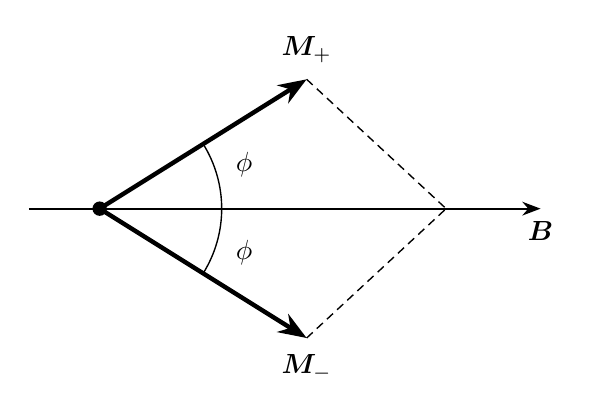
\begin{tikzpicture}[line width=0.8pt,>=Stealth]
\coordinate (O) at (0,0);
% B axis (axis style)
\draw[->,line width=0.8] (-0.9,0) -- (5.6,0) node[below=1pt] {$\bm{B}$};
% origin
\fill (O) circle (2.6pt);
% M+ and M- at +-32 deg
\draw[->,line width=1.6] (O) -- (32:3.1) node[above=2pt] {$\bm{M}_+$};
\draw[->,line width=1.6] (O) -- (-32:3.1) node[below=2pt] {$\bm{M}_-$};
% phi arcs between B and each M
\draw[line width=0.5] (1.55,0) arc[start angle=0,end angle=32,radius=1.55];
\node at (17:1.92) {$\phi$};
\draw[line width=0.5] (1.55,0) arc[start angle=0,end angle=-32,radius=1.55];
\node at (-17:1.92) {$\phi$};
% dashed lines from tips converging onto the B axis
\coordinate (Tp) at (32:3.1);
\coordinate (Tm) at (-32:3.1);
\draw[dash pattern=on 3pt off 2pt,line width=0.5] (Tp) -- (4.4,0);
\draw[dash pattern=on 3pt off 2pt,line width=0.5] (Tm) -- (4.4,0);
\end{tikzpicture}
\end{document}
